% !TeX root = ../libro.tex
% !TeX encoding = utf8

\chapter{MusicVAE}

Magenta es un proyecto de código abierto cuyo objetivo es el desarrollo de herramientas de \textit{machine learning} para la creación artística, especialmente la creación musical. Estas herramientas se construyen sobre la biblioteca TensorFlow. También han publicado numerosos conjuntos de datos utilizados en el entrenamiento de estas herramientas.

MusicVAE~\cite{roberts2018hierarchical} es un modelo desarrollado por Magenta y cuyo objetivo es la codificación y generación de melodías musicales. Se basa en un \textit{autoencoder} variacional cuyo codificador y decodificador toman la forma de redes recurrentes para el tratamiento de secuencias.

\section{Modelo}\label{modelo}

Una gran variedad de estructuras de redes neuronales han sido utilizadas como codificador y decodificador de un \textit{autoencoder} variacional. En este caso se han elegido redes recurrentes para desempeñar dicho cometido. El codificador, $q_{\lambda}(\textbf{z}\vert \textbf{x})$ es una red neuronal recurrente que procesa una secuencia de entrada $x = \{\textbf{x}^{(1)},\textbf{x}^{(2)},...,\textbf{x}^{(T)}\}$ y produce una secuencia de estados ocultos $\textbf{h}_1,...,\textbf{h}_T$. Los parámetros de la distribución sobre las variables latentes $\textbf{z}$ son una función de $h_T$. El decodificador $q_{\theta}(\textbf{x}\vert \textbf{z})$ utiliza el vector latente $\textbf{z}$ para generar la configuración inicial de la red recurrente, que produce la secuencia de salida $y = \{\textbf{y}^{(1)},\textbf{y}^{(2)},...,\textbf{y}^{(T)}\}$.

Existen dos principales inconvenientes en esta estructura. El primero es que las redes neuronales recurrentes son por sí mismas un modelo capaz de reconstruir secuencias. En consecuencia el decodificador puede resultar suficiente para producir un modelo efectivo de los datos y podría ignorar las variables latentes para ello. Esto puede implicar que el término de la convergencia de Kullback-Leibler en el ELBO se establezca trivialmente en cero, con lo que el modelo no estaría actuando como un decodificador. El segundo inconveniente es que el modelo debe comprimir una secuencia completa en un único vector latente, lo cuál puede resultar problemático conforme aumenta el tamaño de la secuencia~\cite{bahdanau2014neural}. El modelo tiene en cuenta estas dos limitaciones e incluye modificaciones en su estructura para evitarlas.

\subsection{Codificador bidireccional}

En el codificador $q_{\lambda}(\textbf{z}\vert \textbf{x})$ se utiliza una red LSTM (\autoref{lstm}) bidireccional (\autoref{rnn-bidirec}) de dos capas (\autoref{rnn-deep}). Se procesa la secuencia para obtener dos vectores de estado oculto finales de la segunda capa, $\overrightarrow{\textbf{h}_T}$ y $\overleftarrow{\textbf{h}_T}$. Estos dos vectores son concatenados en un único vector $\textbf{h}_T$ y sirven de entrada para una capa que produce los parámetros de la distribución como

$$\mu = \textbf{W}_{h\mu}\textbf{h}_T + \textbf{b}_\mu$$
$$\sigma = \log (\exp (\textbf{W}_{h \sigma}\textbf{h}_T + \textbf{b}_{\sigma})+1)$$

donde $\textbf{W}_{h\mu}$, $\textbf{W}_{h\sigma}$ son las matrices de pesos y $\textbf{b}_{h\mu}$, $\textbf{b}_{h\sigma}$ los vectores de sesgos de la capa. El tamaño del vector de estado oculto de LSTM es de $2048$ para cada capa y se tienen $512$ dimensiones latentes.

\subsection{Decodificador jerárquico}

En el decodificador se establece una modificación en la estructura canónica de una red recurrente para obtener mejores resultados en el muestreo y reconstrucción de secuencias largas, mitigando los problemas vistos en la \autoref{modelo}.

La estructura propuesta es la de un decodificador recurrente jerárquico. Asumiendo que la secuencia de entrada $x$ (y también la secuencia objetivo de salida) puede segmentarse en $U$ subsecuencias no superpuestas $y_u$ con final en el punto $i_u$, tales que $$y_u = \{ x_{i_u}, x_{i_u + 1}, x_{i_u + 2},....,x_{i_{u + 1}-1}\},$$ $$x = \{y_1, y_2, ..., y_U \} $$ donde se define el caso especial $i_{U+1} = T$. El vector latente $\textbf{z}$ pasa a través de una capa con función de activación $tanh$ para obtener el estado inicial de una red recurrente "directora". La red directora produce $U$ vectores $c = \{ \textbf{c}_1,...,\textbf{c}_U\}$, uno por cada subsecuencia. Para la red directora se utiliza una red recurrente LSTM de dos capas unidireccional con tamaño de estado oculto de $1024$ y dimensión de salida de $512$.

Una vez que la capa directora produce la secuencia de vectores $c$, cada uno es tratado individualmente por una capa compartida con función de activación $tanh$ que produce los estados iniciales para una última capa recurrente de decodificación. Esta capa produce una secuencia de distribuciones sobre cada unidad de información (\textit{token}) de la salida, en este caso sobre cada corchea para cada subsecuencia $y_u$ mediante una capa de salida softmax. En cada paso de esta última capa de decodificación el vector $\textbf{c}_u$ de la capa directora correspondiente se concatena con el $\textit{token}$ anterior para ser utilizados como entrada. Para este proceso se usan dos capas de LSTM con 1024 unidades por capa.

Al limitar la capacidad del decodificador de transmitir información se le fuerza a que utilice la información de los vectores latentes. En este caso la única manera que tiene el decodificador de obtener información a largo plazo es mediante los vectores obtenidos de la capa directora, que depende directamente de los vectores latentes.

\subsection{Modelo para múltiples secuencias}

A diferencia de otras fuentes de datos secuenciales, como textos, en los que solo existe una secuencia simultánea, en la música normalmente se combinan múltiples secuencias (como múltiples intérpretes tocando diferentes partes o instrumentos de una canción a la vez). Es por ello que MusicVAE incluye también un modelo como el descrito, pero que produce tres secuencias simultáneas: percusión, bajo y melodía. Para ello en la salida se producen tres distribuciones separadas para cada uno de los instrumentos. Cada una de estas distribuciones se produce mediante un decodificador diferente.

\begin{figure}[htpb]
  \centering
  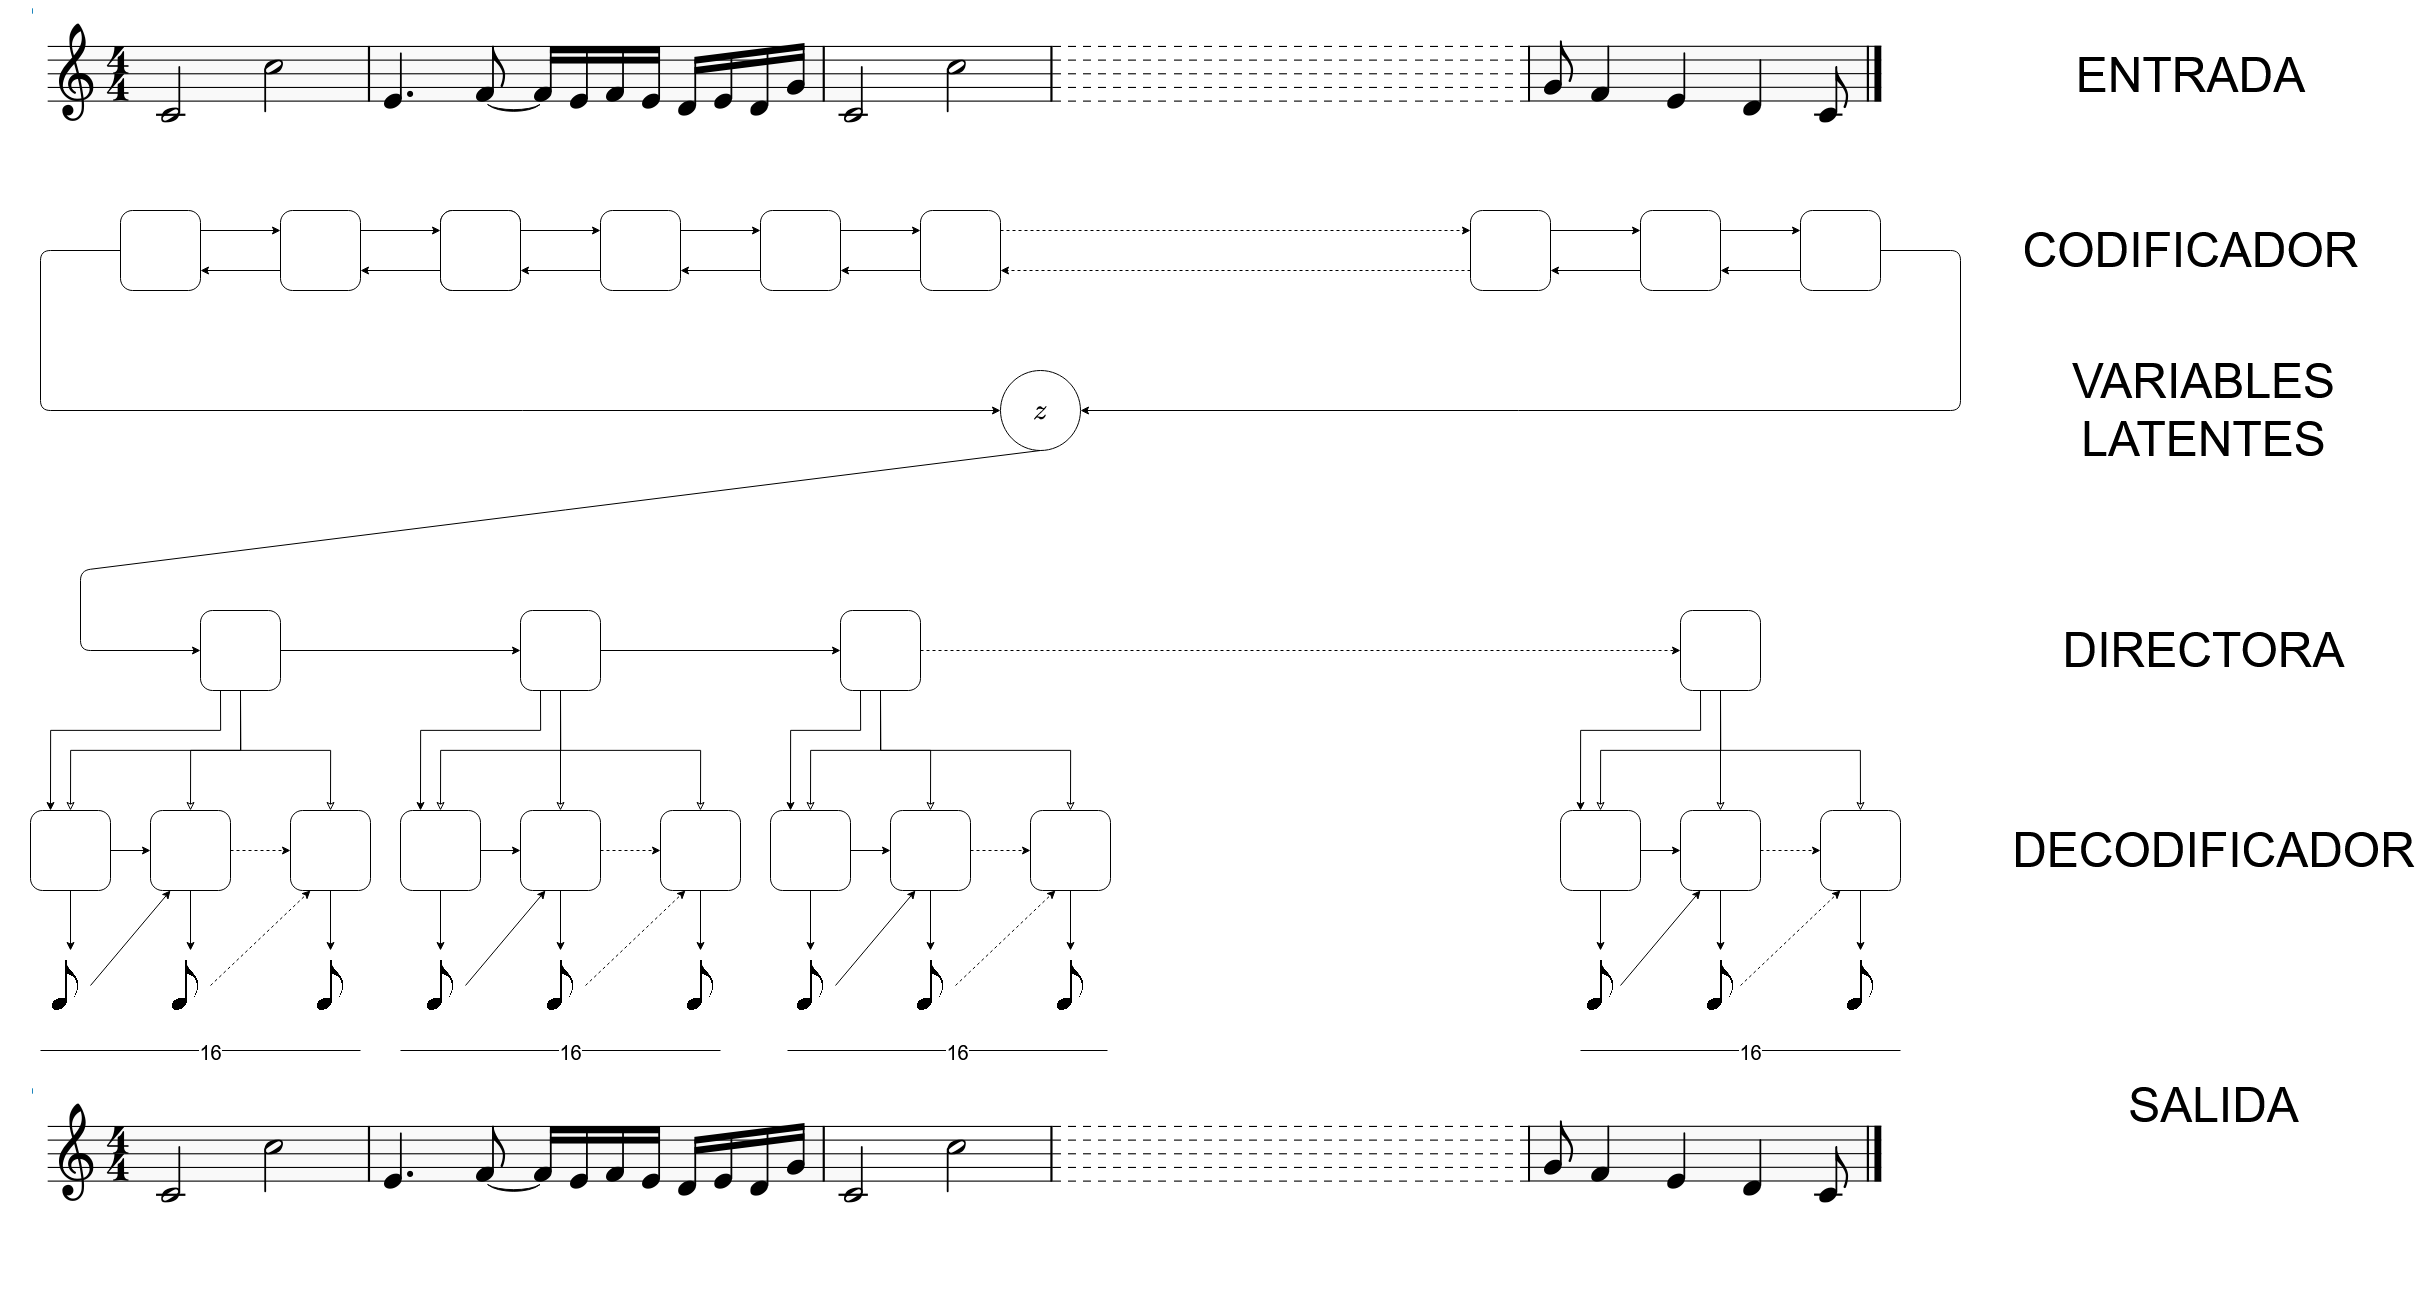
\includegraphics[width=1.1\textwidth]{musicvae}
  \caption{Estructura del modelo MusicVAE}
  \label{fig:musicvae}
\end{figure}


\section{Entrenamiento}

Para el entrenamiento se utilizaron archivos MIDI, que contienen instrucciones para que pueda ser reproducida cada nota de cada instrumento de una canción, así como información de medida (del tiempo). Fueron usados alrededor de 1,5 millones de estos archivos, de los cuales fueron extraídas melodías de 2 compases, melodías de 16 compases, percusiones de 2 y 16 compases y tríos (melodía, percusión y bajo) de 16 compases. Todos los archivos utilizados se encuentran en el compás de 4/4 y la unidad mínima de información considerada es la corchea (un dieciseisavo de compás). En total se obtuvieron $28$ millones de ejemplos diferentes para melodías de dos compases, $19,5$ millones para melodías de dieciséis compases, $3,8$ millones para percusiones de dos compases, $11,4$ millones para percusiones de dieciséis compases y $9,4$ millones para tríos.

Las melodías monofónicas se modelaron con un espacio de salida de dimensión $130$, con $128$ dimensiones representando el evento de ``pulsar una nota'' para cada uno de los $128$ tonos contemplados, un evento de ``dejar de tocar una nota'' y un evento de ``silencio''. Para la percusión se agruparon las sesenta y una clases de percusión del standard MIDI en 9 clases y se representaron todas las posibles combinaciones de golpes con 512 elementos categóricos. En ambos casos se consideran dieciséis eventos por compás, por lo que para los datos de dos compases se tiene $T = 32$ y para los de dieciséis compases se tiene $T = 256$. En todos los casos se utiliza $U = 16$, por lo que cada subsecuencia representa un compás completo. Todos los modelos se entrenan mediante el algoritmo Adam (\ref{adam}) con una tasa de aprendizaje entre $10^{-3}$ y $10^{-5}$, con ratio de decaimiento exponencial de $0,9999$ y tamaño de lotes de $512$. Los modelos de dos compases se entrenaron con $50000$ actualizaciones del gradiente y los de dieciséis compases con $100000$.

\section{Propiedades}

De la utilización del espacio latente para la representación de melodías se derivan ciertas propiedades que pueden ser explotadas en la utilización creativa de la herramienta que supone el modelo para la generación de música.

\subsection{Interpolación}\label{interpolate}

Dado un punto del espacio latente que se identifica con un dato real, los puntos cercanos en el espacio latente deberían corresponderse con datos reales parecidos. Esto implica que todos los puntos a través de una curva continua que conecta dos puntos en el espacio latente deberían ser identificables a una serie de ejemplos reales que produzcan una interpolación suave entre los ejemplos de los extremos. Para ello se requiere que el espacio latente no tenga regiones que no se identifiquen con ejemplos realistas. Estos requerimientos deberían cumplirse si ambos términos del ELBO son suficientemente bajos.

Una comprobación práctica de esta propiedad es realizar una interpolación entre puntos del espacio latente y comprobar si el resultado con sus correspondientes datos reales es adecuado. Dados $\textbf{z}_1$ y $\textbf{z}_2$ vectores latentes correspondientes a los datos $\textbf{x}_1$ y $\textbf{x}_2$, se puede realizar la interpolación lineal $$\textbf{c}_{\alpha} = \alpha \textbf{z}_1 + (1 - \alpha)\textbf{z}_2$$ para $\alpha \in [0,1]$. Se realizará la interpolación satisfactoriamente si para todo $\alpha$ el punto $p_\theta(\textbf{x} \vert \textbf{c}_\alpha)$ es un punto realista y la transición entre $p_\theta(\textbf{x} \vert \textbf{c}_0)$ y $p_\theta(\textbf{x} \vert \textbf{c}_1)$ se realiza de manera suave conforme se varía $\alpha$.

\subsection{Aritmética de vectores de atributos}

Otra propiedad deseada es la obtención de vectores de atributos, que son calculados como la media de los vectores latentes con una determinada característica. Si el modelo es capaz de generar dichos vectores, entonces podría cargarse un ejemplo con determinada característica y, sustrayendo el atributo correspondiente a dicha característica, eliminarla del dato real. Este mismo proceso debe poder realizarse para añadir una característica, sumando el vector de atributo.

Durante los experimentos realizados con el modelo se tomaron cinco características que pueden ser medidas en las melodías: pertenencia a las escala de Do diatónica, densidad de notas, intervalo medio y presencia de síncopas en la subdivisión de corcheas y semicorcheas. Las características fueron medidos en conjuntos de 370000 ejemplos y para cada una el conjunto fue ordenado en función de la cantidad de presencia del atributo. Se dividió entonces el conjunto en cuartiles y se calculó el vector del atributo restando a la media del vector lantente cuartil superior la media del vector latente del cuartil inferior. Después de generaron $256$ muestras aleatorias y se comprobó que sumar el vector obtenido producía un aumento en la característica correspondiente para la melodía. De igual manera la sustracción del vector producía una reducción en la medida de dicha característica.

\endinput
%------------------------------------------------------------------------------------
% FIN DEL CAPÍTULO.
%------------------------------------------------------------------------------------
